
%%%%%%%%%%%%%%%%% Introduction to the Assignment %%%

In this Assignment, \textit{\textbf{Problem 5 - Optimization of phased array antenna radiation pattern and array configuration}}, a phased array consisting of 64 lined up isotropic antennas shall be configured and its configuration investigated. The antenna beam shall be a composite vertical beam in vertical direction, with a operating frequency of 53 MHz.

The design shall be done according to the given equation \ref{eq:orig} in Röttger, chap. 2.1 \citep{roettger1989instrumental}.

\begin{equation}
	E(\delta) = \sum_{n=1}^N E_n(\delta) \exp \Bigg(i\Big(\sin(\delta)\frac{2 \pi (n-1)d}{\lambda}  + \varphi_n \Big)\Bigg)
	\label{eq:orig}
\end{equation}

Additionally, the variables of the design shall be investigated and proper values found.

%%%%%%%%%%%%%%%%% TASK intro %%%
\section{Array Factor Derivation}
\label{chap:derivation}
To understand the different implications of the variables of the given equation \ref{eq:orig}, it is helpful to derive the equation. Also one should take into account the pattern multiplication theorem \citep{donohoe:lecture}, where the array pattern is given as product of each array element pattern times the array factor (AF).
Based on the given boundary condition to use an isotropic radiator (located at origin), the initial equation to start with is the one for the (far) field of an isotropic radiator

\begin{equation}
	E = I_0 \frac{e^{-jkr}}{4\pi r}
	\label{eq:iso_radiator}
\end{equation}
with $I_0$ as current on the antenna, $k$ as wavenumber given by $k = \frac{2\pi}{\lambda}$ and $r$ the distance to the target.
Assuming that the current magnitudes of the array elements are equal, and using the first (origin) array element as phase reference, means this array element has $\varphi = 0$ \citep{donohoe:lecture}, the currents on the array elements are as follows:

\begin{equation}
	I_1 = I_0 , \quad I_2 = I_0 \exp(j \varphi_{2}), \quad \dots \quad I_N = I_o \exp(j \varphi_{N})
	\label{eq:currents}
\end{equation}
with $N$ being the number of array elements.

The distance to the target for each array element can be easily derived using simple geometry (c.f. fig. \ref{fig:radiationPattern}).

\begin{figure}[!h]
\centering
	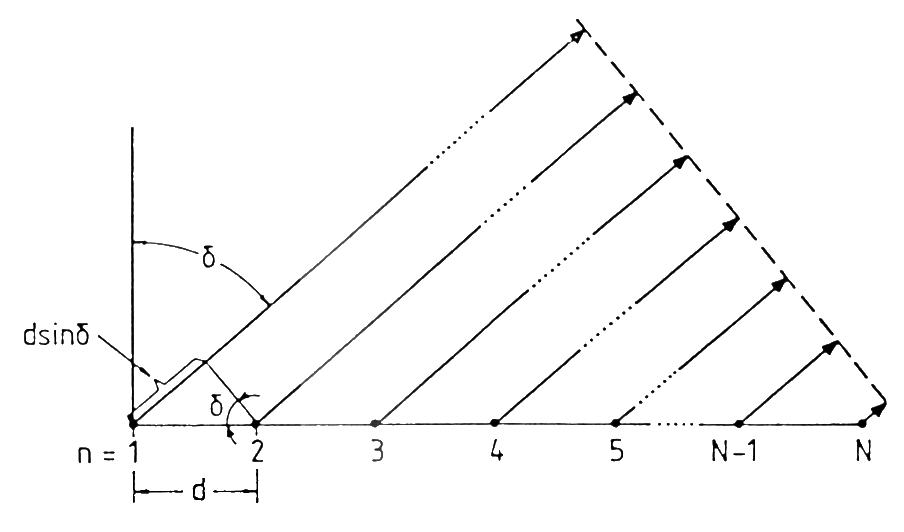
\includegraphics[width=0.7\textwidth]{images/PAradiationPattern}
	\caption{Wave vectors radiated from isotropic antenna elements with spacing d under zenith angle $\delta$ \citep[c.f.][Figure 10]{roettger1989instrumental}}
	\label{fig:radiationPattern}
\end{figure}

Combining the different distances to the targets with the appropriate current for each array element and inserting it into equation \ref{eq:iso_radiator} leads to the radiation pattern for each antenna, denoted in eq. \ref{eq:fieldsOfArray}. 

%\begin{equation}
\begin{eqnarray}
	E_1(\delta) &=& I_0 \frac{e^{-jkr}}{4\pi r}\\
        &\vdots& \nonumber \\
	E_N(\delta) &=& I_0 e^{j\varphi_{N}} \frac{e^{-jk[r - (N-1)d\sin\delta]}}{4\pi r}
	\label{eq:fieldsOfArray}
\end{eqnarray}
%\end{equation}

Assuming that all array element antennas are the same and have the same pattern, the fields can be summed using the superposition principle, to obtain the Array Pattern. Thus using equation \ref{eq:iso_radiator} we can obtain


\begin{eqnarray}
	E_\delta &=& E_1(\delta) + \dots + E_N(\delta) \\
	 &=& E_0 [1 + e^{j\varphi_2 + k d \sin \delta} + \dots + e^{j[\varphi_N + (N-1) k d \sin \delta]}]
\end{eqnarray}

By assuming that the Array Element Pattern $E_0$ for each elements is constant, the Array Pattern will only be affected by the Array Factor. Thus, by applying the substitution $\gamma = \varphi + kd\sin\delta$ we can rewrite the Array Factor as follows:
\begin{equation}
	AF = \sum_{n=1}^N e^{j(n-1)\gamma}
\end{equation}
Multiplying both sides with $e^{j\gamma}$, we can get rid off of the subtraction on the right side, and by subtracting the Array Factor from both sides, we can free the equation from the sum on the right side, which gives us the following expression for the Array Factor:
\begin{equation}
	AF = \frac{e^{jN\gamma} - 1}{e^{j\gamma} - 1} = e^{0.5j(N-1)\gamma} \frac{\sin(\frac{N\gamma}{2} )}{\sin(\frac{\gamma}{2} )}
\end{equation}

If we now shift the position of the array, so that the center of the is located at $N = 1$ (which represents a shift by $-\varphi$), the complex exponential expression reduces to 1. Inserting the re-substitution and expressing the wavenumber with $k = \frac{2\pi}{\lambda}$, we get the following real expression for the Array Factor:
\begin{equation}
	AF = \frac{\sin(\frac{Nd\pi\sin\delta}{\lambda})}{\sin(\frac{d\pi\sin\delta}{\lambda})}
	\label{eq:AF}
\end{equation}

%%%%%%%%%%%%%%%%% TASK 1 %%%
\section{Optimal distance between array elements}
Using the derived Array Factor equation in chap. \ref{chap:derivation}, the Array Pattern can be plotted using Matlab (). The Array Factor was normalized to the number of Array Elements, to be able to compare the results in an easier way.

\begin{figure}[h!]
	\centering
	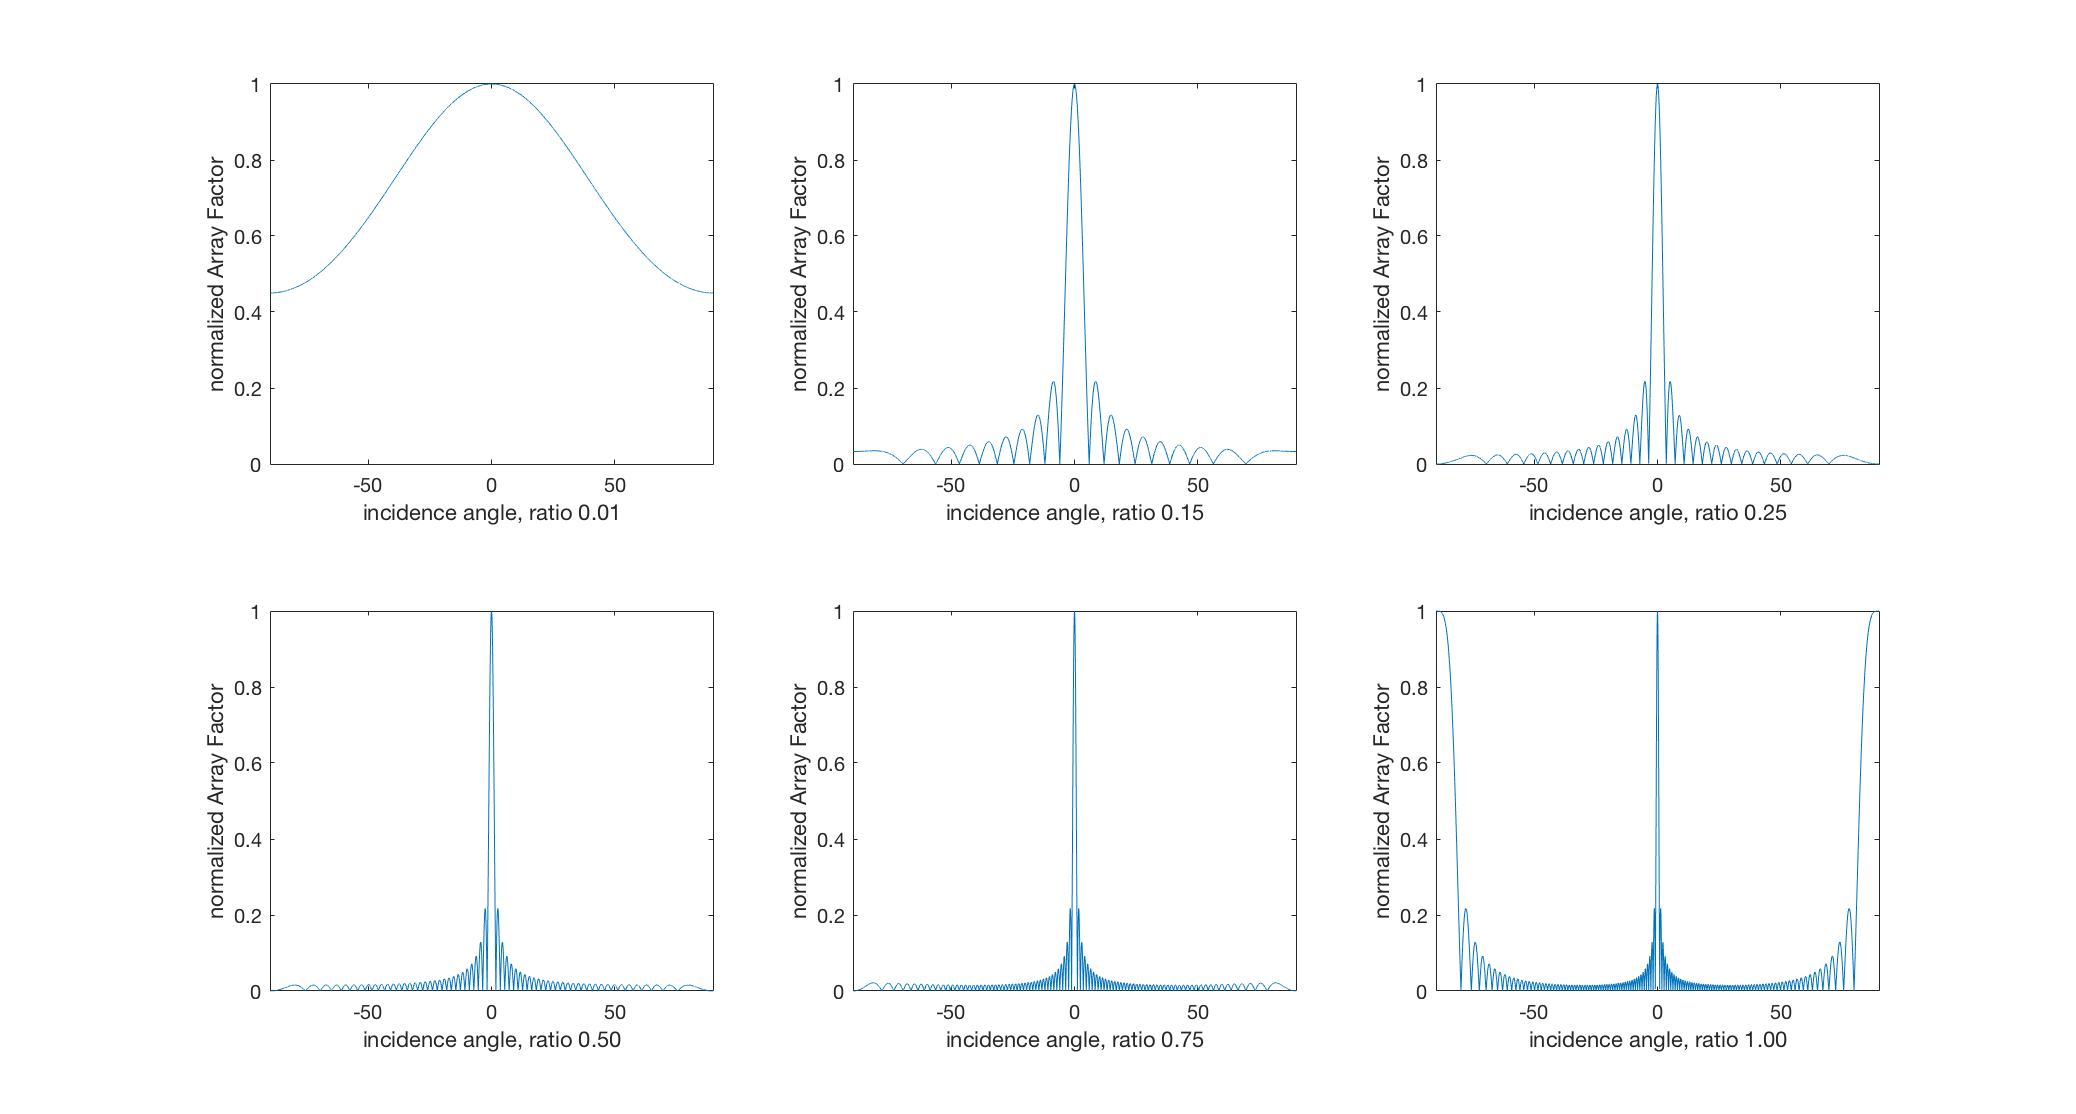
\includegraphics[width=\textwidth]{images/distanceVariation}
	\caption{Array Pattern with various distance-to-wavelength ratios}
	\label{fig:distance}
\end{figure} 

According to Richards et. al. \citep{richards2010principles}, the maximum allowable distance between the array elements must fulfil the equation
\begin{equation}
	\Delta x \leq \frac{\lambda}{(1 + |\sin\theta_S |)}
	\label{eq:deltaX}
\end{equation}

with $\theta_S $ being the desired maximum scan angle of the phased array. Inserting the appropriate values for the given antenna parameters leads to a ideal spacing of 2.8826m, which corresponds to an ideal distance-to-wavelength ratio of 0.5. The maximum spacing between two adjacent antennas is seen as ideal, since this minimizes the cost of the antenna setup and electronics \citep{richards2010principles}, but is still small enough so that grating lobes are pushed outside the scan window.

%%%%%%%%%%%%%%%%% TASK 2 %%%
\section{Number of antenna elements}
Using again the Array Factor equation \ref{eq:AF}, the number of array Elements is varied and the resulting (normalized) Array Factor is plotted against the scanning angle. For these plots the distance-to-wavelength was set to 0.5, according to the results from the previous chapter. As one can see in fig. \ref{fig:varyingElements}, the main lobe gets "sharper" and thinner, the more Array Elements are used. But we also get more sidelobes the more Array Elements we have.

\begin{figure}[h!]
	\centering
	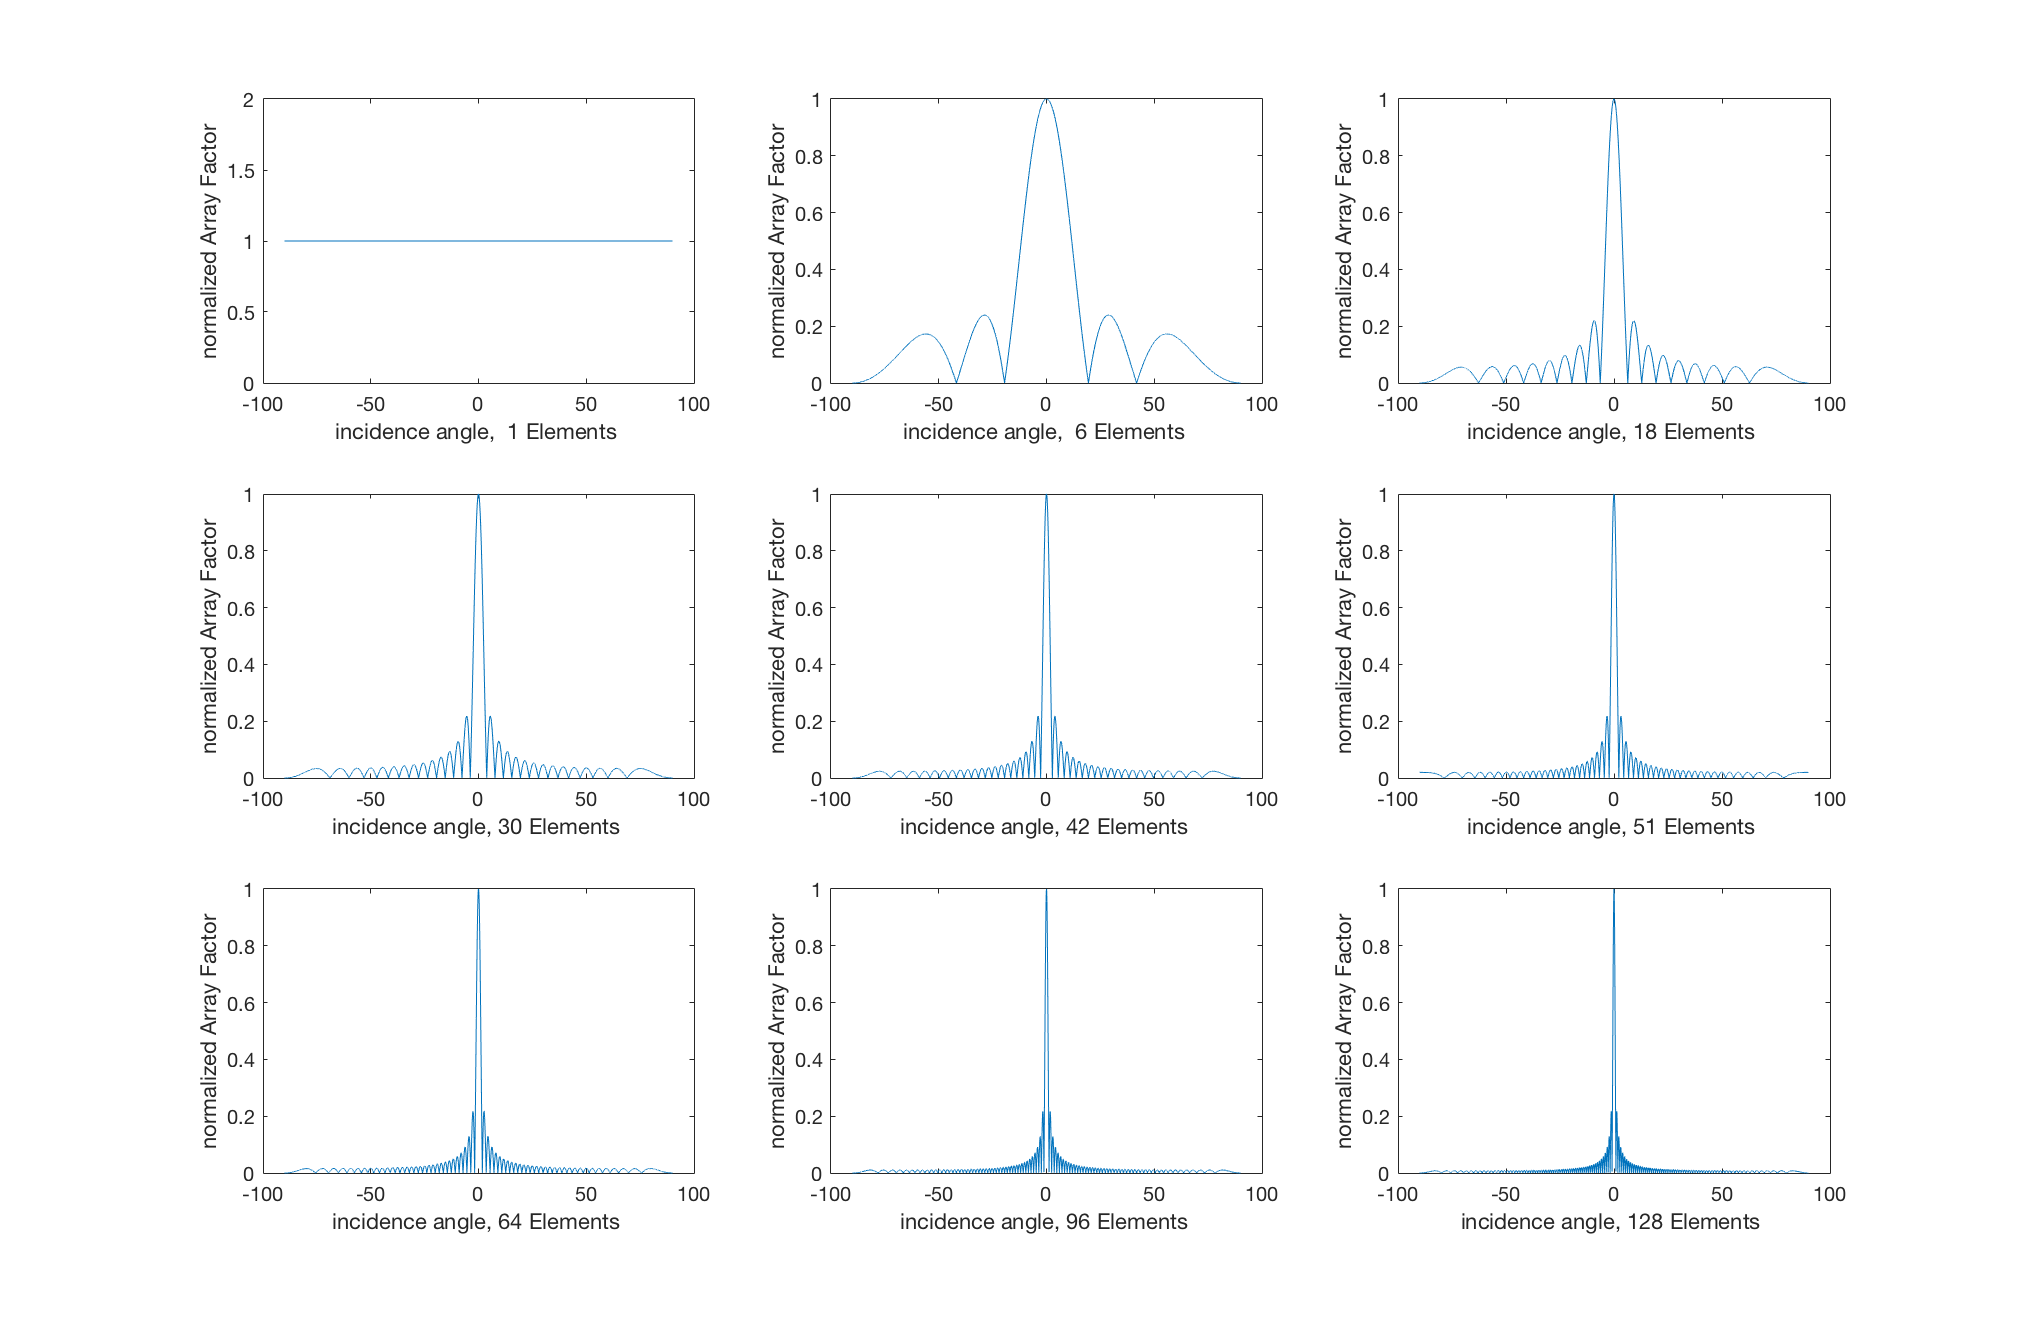
\includegraphics[width=\textwidth]{images/elementVariation}
	\caption{varying amount of array elements, with fixed $\frac{d}{\lambda}$-ratio of 0.5}
	\label{fig:varyingElements}
\end{figure}



%%%%%%%%%%%%%%%%% TASK 3 %%%
\section{Spatial Weighting}
To further suppress the side lobes, one can apply a technique called "spatial weighting". Here, the distance between the elements is increased, starting from the middle of the antenna.\todo{language}
Since now the distance between the Array Elements are not uniform, and thus the phase shift in-between is neither, we can not use the simplified equation \ref{eq:AF}, derived in chapter \ref{chap:derivation}, but must use the initially given expression in \ref{eq:orig} \citep{roettger1989instrumental}.

\begin{figure}[h!]
	\centering
	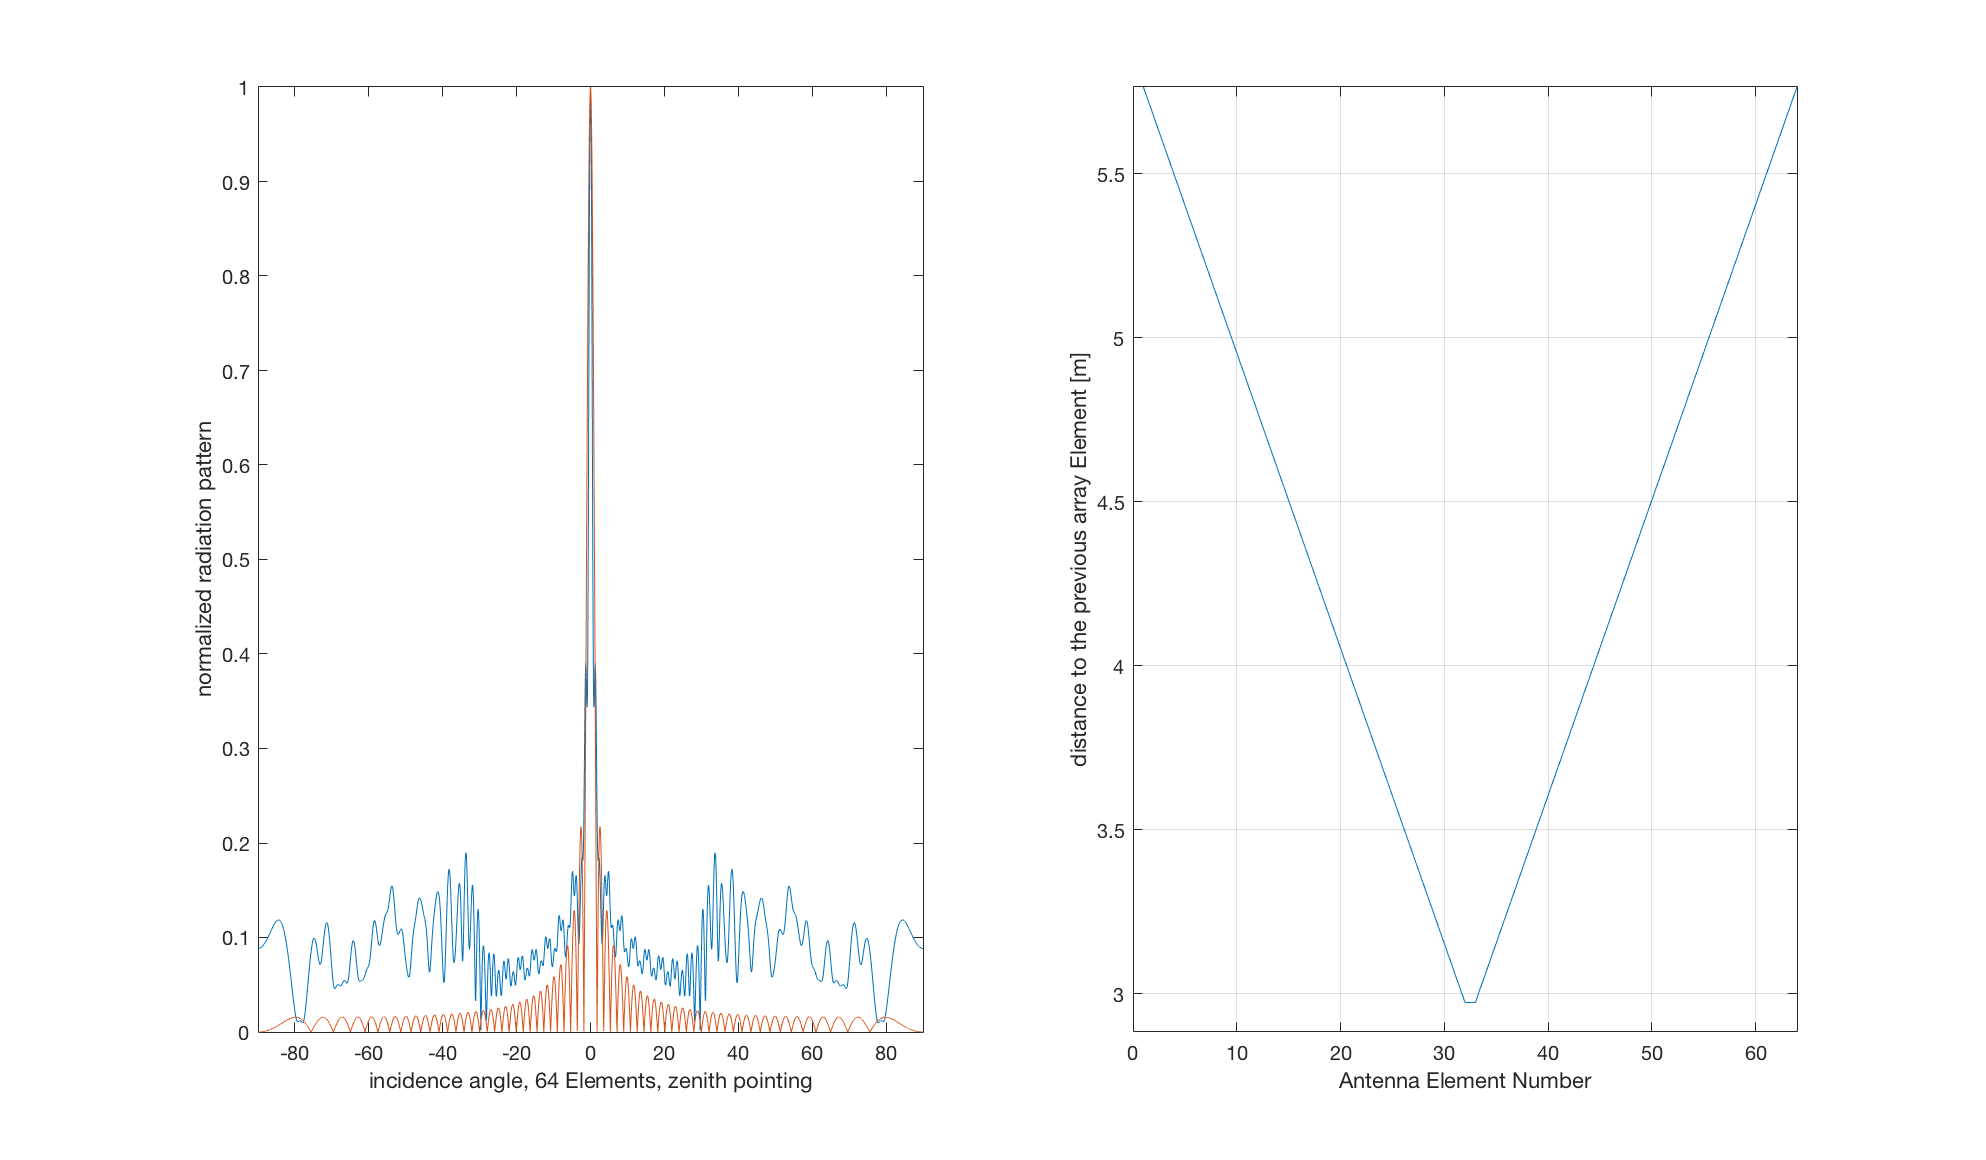
\includegraphics[width=\textwidth]{images/triangularSpatialWeight}
	\caption{Spatial Weighting for Array Elements}
	\label{fig:triangWeight}
\end{figure}

Comparing fig. \ref{fig:triangWeight} with fig. \ref{fig:varyingElements} (64 Elements), we can see, that the sidelobes right next to the main lobe are heavily suppressed when a triangular weighting function is used, to increase the distance in the outer elements. However, this introduces an increase of sidelobe amplitudes in higher incidence angles, which might not be desired in all applications.



%%%%%%%%%%%%%%%%% TASK 4 %%%
\section{Optimal Design for antenna array}
\label{chap:optimal}
Taking into account the results of the previous chapters, we can conclude, that with the given antenna parameters, 64 lined up isotropic antennas, 53MHz operating frequency and a beam pointing in zenith angle, the optimal design parameters would be as follows:
The optimal distance-to-wavelength-ratio would be 0.5, to push the sidelobes further outside.
The number of of the lined up antennas 64, since it was given as an initial parameter.
Also, the spatial weighting would not be done, since this introduces high sidelobes on the outer scanning angles and only suppresses the direct lobes next to the main lobe, only for a limited amount.

%%%%%%%%%%%%%%%%% TASK 5 %%%
\section{Main lobe maximum and width}
The main lobe is located at an incidence angle $\delta = 0$. 
The maximum of the main lobe can be calculated by applying the limit $$\lim_{x\to0} \frac{\sin(Nx)}{\sin(x)} = N $$ by using the Taylor-Expansion (c.f. Seminar 5).
Also, we can easily see this by plugging in the main lobe angle of 0° in eq. \ref{eq:orig}, which simplifies to
\begin{equation}
	E(0) = \sum_{n=1}^N E_n(0)
\end{equation}
In our case, the maximum of the main lobe is 64 Power Units, since the exact maximum depends on the Array Element Pattern and its unit, which, in this case, was set to 1.
According to Röttger et. al. \citep{roettger1989instrumental} main lobe width can be calculated using eq. \ref{eq:AF}
\begin{equation}
	\varphi_{B} = \arcsin(\frac{\lambda}{Nd})
\end{equation}

where $d$ is the distance between array elements and $N$ the number of array elements Array Elements. This gives us a main lobe width of $\varphi_{3dB} = 1.7908$°.


%%%%%%%%%%%%%%%%% TASK 6 %%%
\section{Radiation pattern change at non-vertical beam}
To provide a different beam pointing than the vertical one, we must take into account the phase shifts between the array elements. The phase shifts between the origin and n-th element can be calculated as follows \citep{richards2010principles}:
\begin{equation}
	\varphi_n = \frac{2\pi n}{\lambda}d \sin(\delta)
	\label{eq:pointing}
\end{equation}

Inserting eq. \ref{eq:pointing} in eq. \ref{eq:orig} gives us eq.\ref{eq:pointingSum} and plotting leads to fig. \ref{fig:pointing}.

\begin{equation}
	E(\delta) = \sum_{n=1}^N E_n(\delta) \exp \Bigg(-i\Big(\frac{2 \pi nd}{\lambda} (\sin(\delta) - \sin(\delta_s)) \Big)\Bigg)
	\label{eq:pointingSum}
\end{equation}
with $\delta_s$ as the wanted beam direction angle.

We can easily see, that steering the antenna in different directions moves the main lobe to the desired angle, while the beam width gets bigger the more the antenna is steered. According to Richards et. al.\citep{richards2010principles} the beam magnitude also gets lower in a real system, due to imperfections in the phase shifters. But in theory, as we can see in the mentioned figure, the main lobe magnitude stays the same.

\begin{figure}[h!]
	\centering
	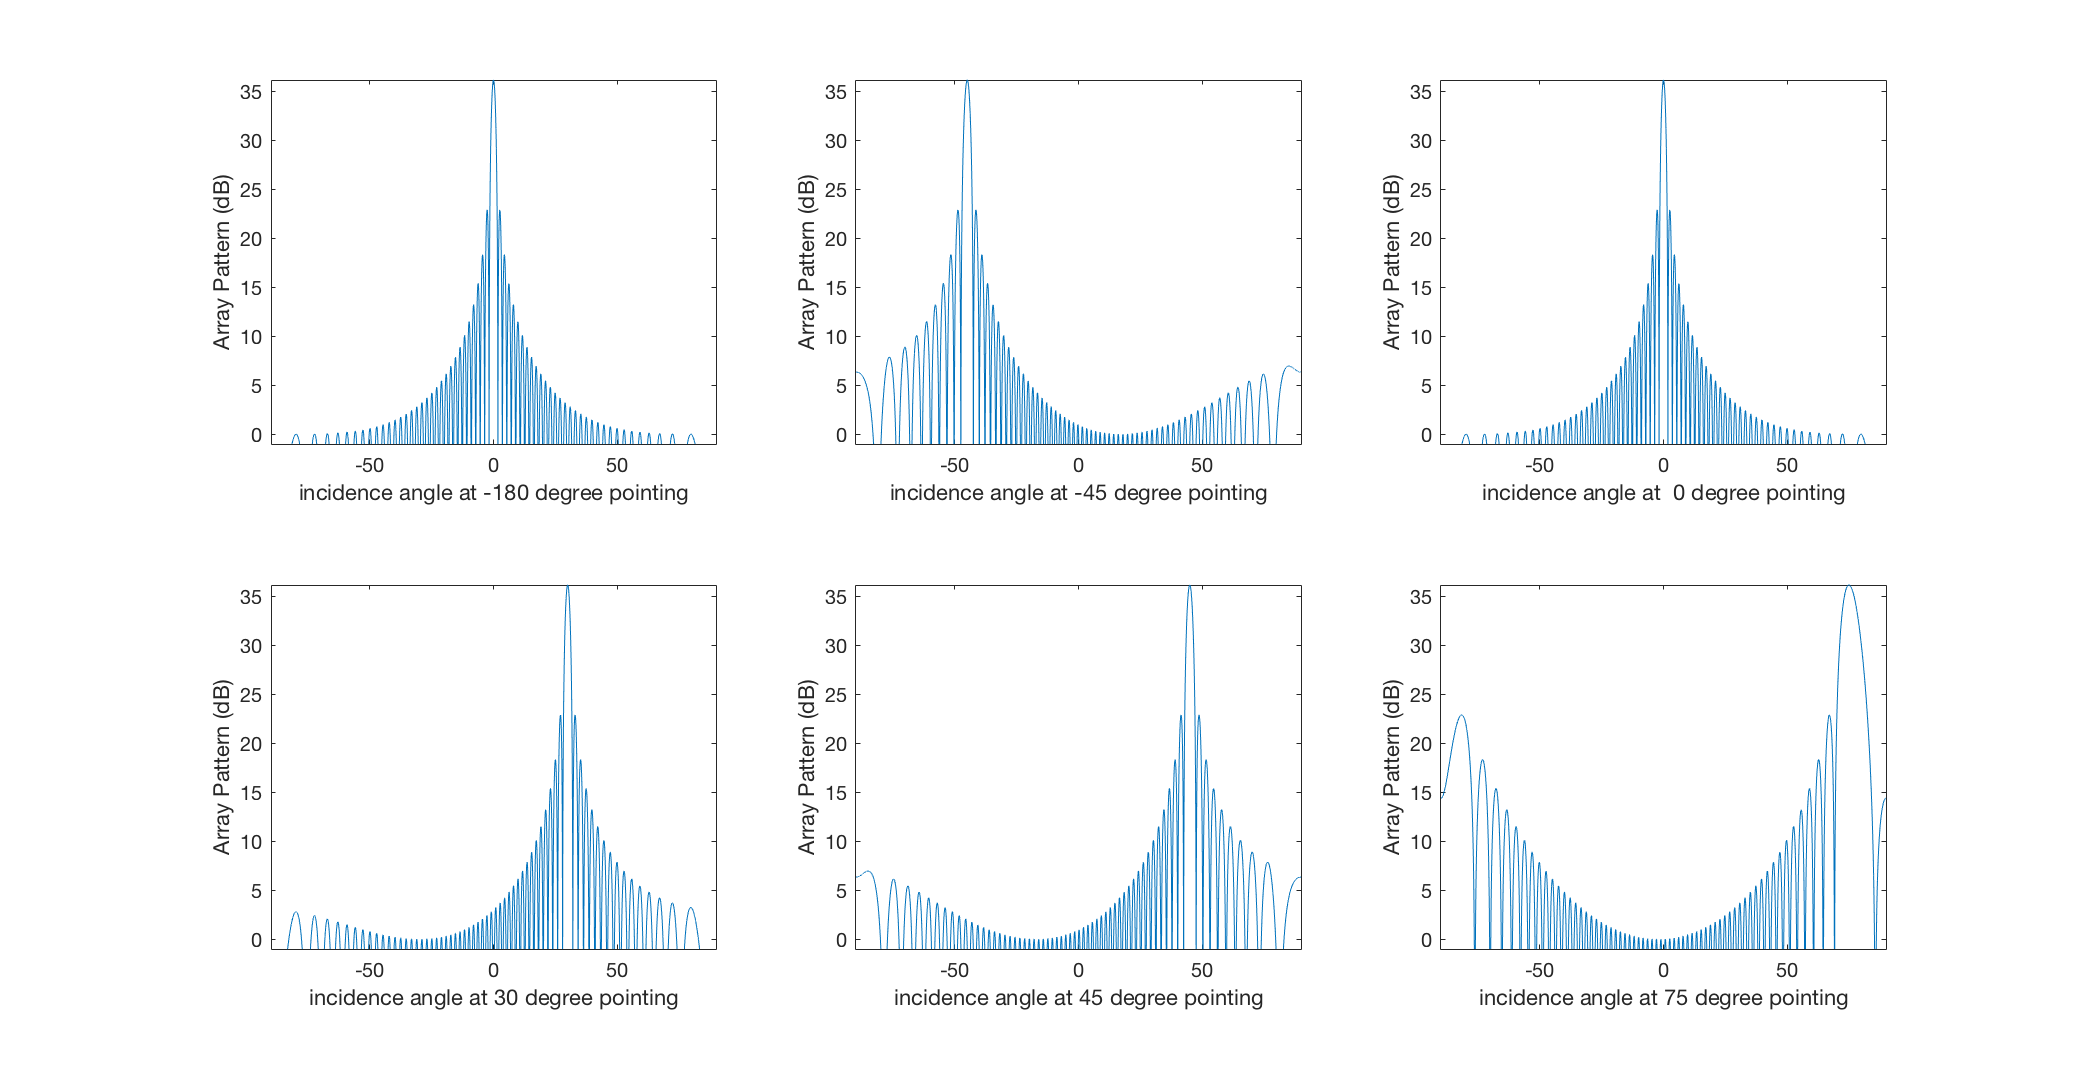
\includegraphics[width=\textwidth]{images/variablePointing}
	\caption{different beam pointings}
	\label{fig:pointing}
\end{figure}


%%%%%%%%%%%%%%%%% TASK 7 %%%
\section{Electrical Weighting}
\begin{figure}[h!]
	\centering
	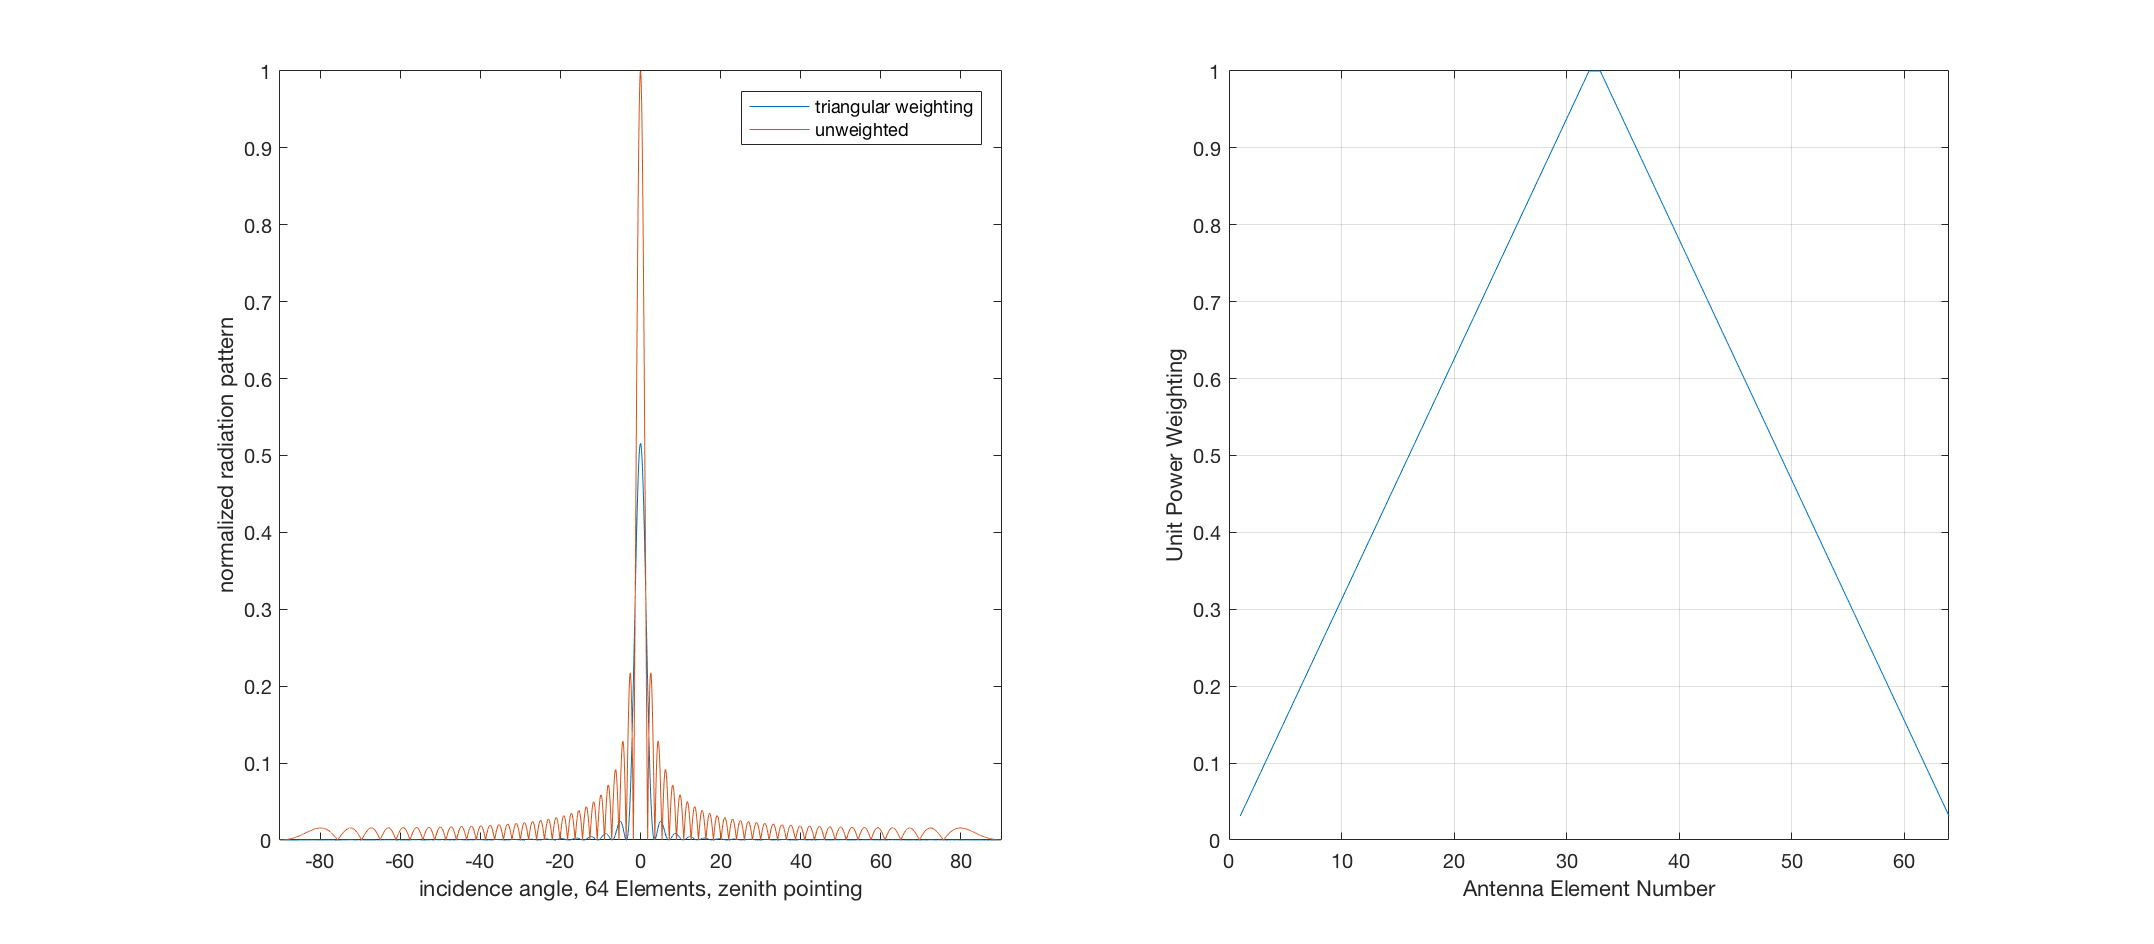
\includegraphics[width=\textwidth]{images/triangularElectricalWeight}
		\caption{Electrical Weighting with Triangular Function}
	\label{fig:electricalWeight}
\end{figure}

Electrical Weighting is a technique to lower the amplitude of side-lobes by feeding the outer array elements with less power than the inner ones. This can be done by applying a weighting function to the Array Element Pattern.
To visualize the impact of electrical weighting, fig. \ref{fig:electricalWeight} shows the Array Pattern after applying a simple triangular weighting function to the Array Element Pattern, by using the in chap. \ref{chap:optimal} mentioned optimal array parameters, such as a $\frac{d}{\lambda}$-ratio of 0.5, no spatial weighting, 64 Array Elements and a vertical beam (0° pointing).
The appropriate MATLAB-Code can be found in Appendix \ref{apdx:matlab}.

As one can see in the figure, the main lobe is heavily reduced when electrical weighting is applied, but also the side lobes are heavily attenuated with a factor greater than 2, which means that the sidelobes are more attenuated than the main lobe.

Depending on the application, this electrical weighting technique could be very useful, if the power margin calculated such as half the power would still be enough for the appropriate targets.


